\documentclass[../VorlesungMaster.tex]{subfiles}
\begin{document}
	
%Vorlesung8 14.11.17
\subsection{Güte der Schätzungen für $\beta_0$ und $\beta_1$}
Beachten Sie, Der wahre Zusammenhang zwischen Y und X ist unbekannt d.h. die wahre Regressionsgerade ist unbekannt. \\
\textbf{Grund:} 
\begin{itemize}
	\item Schätzungen für $\hat{\beta_0}$ und$ \hat{\beta_1}$ hängen von der gewählten Trainingsmenge ab\\
\end{itemize}
\textbf{Daraus Folgt:} 
\begin{itemize}
	\item Die geschätzten Regressionsgeraden schwanken um die wahre Regressionsgerade.
	\item Koeffizienten $\beta_0$ und $\beta_1$ sind Zufallsvariablen, welche auf Basis der gezogengen Beobachtungen $(x_i,y_i)$ geschätzt werden.
\end{itemize}


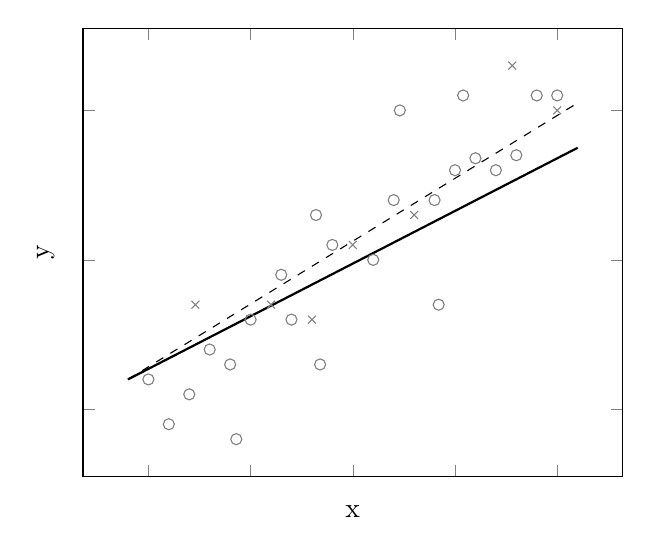
\begin{tikzpicture}
\begin{axis}[%
scatter/classes={%
	a={mark=o,draw=gray},
	b={mark=x,draw=gray}},
xlabel={x},
ylabel={y},
xticklabels={,,},
yticklabels={,,}
]
\addplot[scatter,only marks,%
scatter src=explicit symbolic]%
table[meta=label] {
	x y label
	10 12 a
	11 9 a
	12 11 a
	12.3 17 b
	13 14 a
	14 13 a
	14.3 8 a
	15 16 a
	16 17 b
	16.5 19 a
	17 16 a
	18 16 b
	18.2 23 a
	18.4 13 a
	19 21 a
	20 21 b
	21 20 a
	22 24 a
	22.3 30 a
	23 23 b
	24 24 a
	24.2 17 a
	25 26 a
	25.4 31 a
	26 26.8 a
	27 26 a
	27.8 33 b
	28 27 a
	29 31 a
	30 30 b
	30 31 a
};
\addplot [thick] coordinates { (9,12) (31,27.5) };
\addplot [dashed] coordinates { (9,12) (31,30.5) };
\end{axis}
\end{tikzpicture}




Varianz für $\beta_1$:
\[ 
	Var(\beta_1)= \frac{\sigma_{\epsilon}^2}{\sum\limits_{i=1}^n (x_i-\bar{x})^2} 
\]
mit $\sigma_{\epsilon}^2$ ist die Varianz der Fehler $\epsilon$
\[\sigma_{\epsilon}^2 = \frac{RSS}{n-2} \]

\[\hat{Var}(\beta_1)=\frac{RSS/(n-2)}{\sum\limits_{i=1}^n (x_i-\bar{x})^2} \]
Varianz von $\beta_1$ ist klein, wenn:
\begin{enumerate}
	\item Varianz der Störgrößen klein ist
	\item Stichprobengrößen n groß ist
\end{enumerate}
\[Var(\beta_0) = \frac{\sigma_\epsilon^2  \sum x_i}{n Var(X)}\]
\todo{ $Var(\beta_0)= \frac{ \sigma_{\epsilon}^2 \sum x_i^2}{n Var(X)} $???}

\subsection{Das Bestimmtheitsmaß $R^2$}
Wie gut ist die Schätzung der Daten anhand der gefitteten Geraden. \\
$\Rightarrow$ Schätzung ist dann besonders gut, wenn der Anteil von RSS an Gesamtvarianz(TSS) klein ist und somit die erklärte Varianz möglichst groß ist.

\[ R^2= \frac{\text{erklärbare Varianz}}{\text{Gesamtvarianz}}
= \frac{TSS-RSS}{TSS} = 1 - \frac{RSS}{TSS}\]
\todo{$TSS=\sum(\hat{y}-\bar{y})^2 + RSS$}

\[ 0 \leq R^2 \leq 1\]
$R^2 \approx 1$: Ein großer Anteil der Variabilität in der Zielvariablen durch gelernte Regressionsgerade erklärt. \\
$R^2 \approx 0$: \underline{Kein} großer Anteil der Variabilität in der Zielvariablen durch gelernte Regressionsgerade erklärt.





\subsection{Testen ob es einen signifikanten Zusammenhang zwischen Y und X gibt}
Frage Existiert irgendein Zusammenhang zwischen X und Y, also $\beta_1 \neq 0$\\
$H_0:$ Es existiert kein Zusammenhang $ \Leftrightarrow $ $ \beta_1 = 0$\\
$H_1:$ Es existiert ein Zusammenhang $ \Leftrightarrow $ $\beta_1 \neq 1$\\

Teststaistik: t-Statistik, welche t-Verteilung folgt $t= \frac{\hat{\beta_1}}{s.d.(\hat{\beta_1})} = \frac{\hat{\beta_1}}{\sqrt{Var(\hat{\beta_1})}} \approx t_{1-\alpha/2, n-2}$

$|t| \leq  t_{1-\alpha/2, n-2} \rightarrow H_0$ wird beibehalten

$|t| >  t_{1-\alpha/2, n-2} \rightarrow H_0$ wird abelehnt, wir können annehmen das $\beta_1 \neq 0$


\subsection{Multilinerare lineare Regression}
\begin{itemize}
	\item Erweiterung der einfachen linearen Regression auf mehreren Kovariablen $X=\{{X_1, \ldots, X_p}\}$
	\item Identifiziere ein verbessertes Modell als es auf Basis einer einzelnen Kovariable möglich ist 
	\item Individuelle Effekte der Kovariablen $X_I$ können durch partielle Regressionsgeraden modelliert werden.
	\item  Jede partielle Regressionsgerade entspricht(modelliert) den Effekt von $X_i$ während alle anderen Kovariablen $X_{j \neq i}$ ihren Mittelwert annehmen
\end{itemize}

\subsubsection*{Additives multivariables lineares Regressionsmodell}
Annahme: Effekt einer Kovariablen $X_i$ auf Y ist unabhängig von allen anderen Kovariablen 
\[Y = \beta_0 + \beta_1X_1 + \beta_2X_2 + \ldots + \beta_p X_p + \epsilon\]
$ \beta_1,\ldots,\beta_p$ geben Effekte der Kovariablen $X_1, \ldots, X_p$ auf Y an.\\
p: Anzahl der Kovariablen\\ 
$ \beta_0 $ Mittelwert von Y , falls alle Koeffizienten $ \beta_j = 0 $\\
$\epsilon$ ist der Fehler $\epsilon \sim N(0, \sigma^2)$


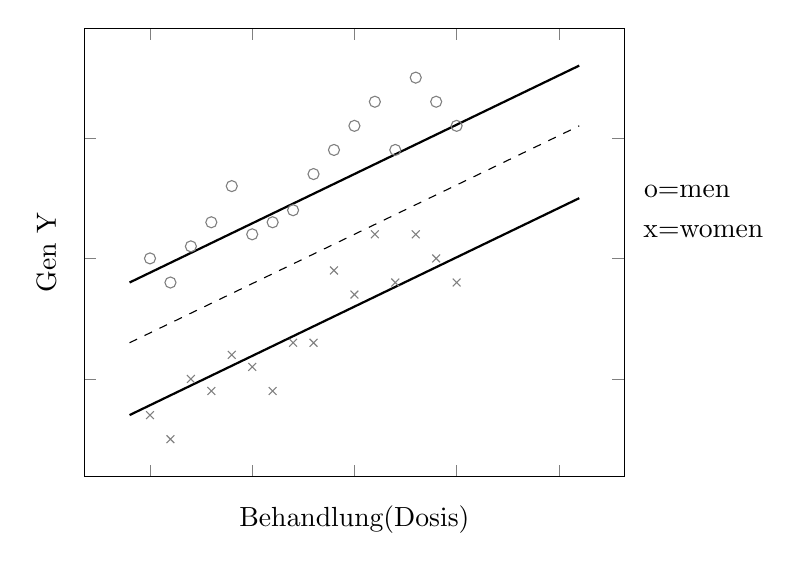
\begin{tikzpicture}
\begin{axis}[%
scatter/classes={%
	a={mark=o,draw=gray},
	b={mark=x,draw=gray}},
ylabel={Gen Y},
xlabel={Behandlung(Dosis)},
xticklabels={,,},
yticklabels={,,}
]
\addplot[scatter,only marks,%
scatter src=explicit symbolic]%
table[meta=label] {
	x y label
	10 20 a
	11 18 a
	12 21 a
	13 23 a
	14 26 a
	15 22 a
	16 23 a
	17 24 a
	18 27 a
	19 29 a
	20 31 a
	21 33 a
	22 29 a
	23 35 a
	24 33 a
	25 31 a
	10 7 b
	11 5 b
	12 10 b
	13 9 b
	14 12 b
	15 11 b
	16 9 b
	17 13 b
	18 13 b
	19 19 b
	20 17 b
	21 22 b
	22 18 b
	23 22 b
	24 20 b
	25 18 b
};
\addplot [thick] coordinates { (9,7) (31,25) };
\addplot [thick] coordinates { (9,18) (31,36) };
\addplot [dashed] coordinates { (9,13) (31,31) };
\end{axis}
\node[] at (rel axis cs:1.23,0.63){x=women};
\node[] at (rel axis cs:1.2,0.72){o=men};
\end{tikzpicture}
\todo{Hoher Fehler mit einfacher Regression (gestrichelt), also additiv nutzen}



\subsection*{Multiplikatives Modell}
\begin{itemize}
	\item Interaktionen zwischen den Kovariablen sind möglich
	\item D.h. partieller Effekt einer Kovariablen $X_i$ kann vom partiellen Effekt von $X_j$ abhängig sein
\end{itemize}
\[Y = \beta_0+ \beta_1X_1 + \beta_2X_2 + \beta_3 X_1X_2 + \beta_4 X_3 +\ldots \beta_{p+1}X_p + \epsilon\]

$\beta_3:$ Gibt an, inwieweit der Effekt von $X_1$ von den Werten von $X_2$ abhängt

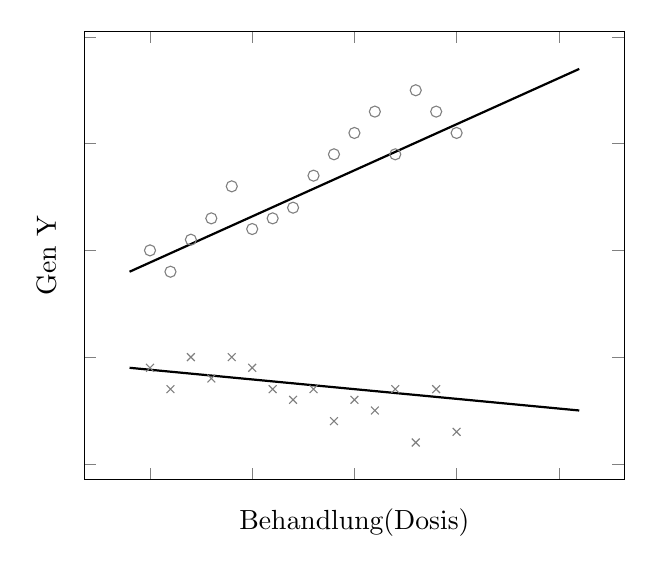
\begin{tikzpicture}
\begin{axis}[%
scatter/classes={%
	a={mark=o,draw=gray},
	b={mark=x,draw=gray}},
ylabel={Gen Y},
xlabel={Behandlung(Dosis)},
xticklabels={,,},
yticklabels={,,}
]
\addplot[scatter,only marks,%
scatter src=explicit symbolic]%
table[meta=label] {
	x y label
	10 20 a
	11 18 a
	12 21 a
	13 23 a
	14 26 a
	15 22 a
	16 23 a
	17 24 a
	18 27 a
	19 29 a
	20 31 a
	21 33 a
	22 29 a
	23 35 a
	24 33 a
	25 31 a
	10 9 b
	11 7 b
	12 10 b
	13 8 b
	14 10 b
	15 9 b
	16 7 b
	17 6 b
	18 7 b
	19 4 b
	20 6 b
	21 5 b
	22 7 b
	23 2 b
	24 7 b
	25 3 b
};
\addplot [thick] coordinates { (9,9) (31,5) };
\addplot [thick] coordinates { (9,18) (31,37) };
\end{axis}
\end{tikzpicture}


\subsection{Schätzung der Koeffizienten $\beta_1 ... \beta_p$}
Methode der kleinsten Quadrate
\[\hat{Y} = \hat{\beta_0} + \hat{\beta_1} X_1 + ... + \hat{\beta_p} X_p \]

\[ RSS = Var(\epsilon)= \sum\limits_{i=1}^n (y_i - \hat{y_i} )^2 \]
\[ \sum (y_i - \hat{\beta_0} - \hat{\beta_1} X_1 - ... - \hat{\beta_p} X_p )^2 \rightarrow min \]
Über partielle Ableitungen werden die Koeffizienten $\beta_i$ geschätzt

\end{document}